%!TEX root = ../thesis.tex
\section{Computer-Generated Mixed Media Tutorials}

The benefits of mixed media tutorials are unlikely to be realized if creating such materials is too tedious, time-consuming, or if it requires more expertise than creating other tutorial formats. To lower the authoring barrier, we designed MixT, a system that automatically generates mixed media tutorials from user demonstrations. While the MixT architecture can apply to different media creation applications, our current implementation is specific to creating tutorials for Adobe Photoshop.

\subsection{Overview}
\subsubsection{Tutorial Format}
MixT generates HTML tutorials with embedded videos that follow the design guidelines identified in our study. By default, our interface presents a textual description and screenshot for each step, just like a standard static tutorial (see Figure~\ref{fig:mixt_teaser}A). Clicking on the screenshot replaces the static image with a video player that plays the segment of the original demonstration that corresponds to the written step instructions. For example, a screenshot of a layer panel enhances the instruction ``\emph{Select Soft Light from the drop-down menu for Blend Mode},'' and the corresponding video clip shows continuous mouse action to the menu, expanding the drop-down menu, moving down to click on the feature, and shows the canvas change. By presenting steps as text and images with video clips that are accessible on demand, MixT tutorials retain the scannability of static tutorials while giving users the option of static- or video-based instruction at each step. To ensure that steps remain scannable and that the tutorial can still be viewed alongside the image editing application (without window switching), we scale each in-place video to at most 700 pixels wide and display text instructions on the left.

\subsubsection{Video Playback Options }
The MixT video player gives users additional control over the format of playback. Three different modes (normal, zoom, and crop) each emphasize different types of information (Figure 6). In addition, users can display a pointer trace visualization to clarify the path of mouse interactions.

\emph{\textbf{Normal mode}} shows the entire application window (Figure~\ref{fig:mixt_modes}A). This mode preserves all context, but because MixT scales videos down to at most 700x440 pixels positioned next to the text instructions, it may be hard to see precise manipulation or small widgets or handles in the UI.

\emph{\textbf{Zoom mode}} also shows the entire application window, but performs a non-uniform enlargement of specific UI regions. In particular, the application area being manipulated (e.g., a menu, dialog, or the canvas) is enlarged to fill the full height of the frame and composited on top of the original video in another video layer (Figure~\ref{fig:mixt_modes}B). If a dialog also modifies pixels on the canvas, both areas are enlarged and positioned such that they do not overlap. This video composition effectively creates a focus-plus-context view that makes important regions easier to see at a given video resolution \cite{Furnas:1986:GFV:22627.22342}. Commercial screencasting software commonly includes a pan-and-zoom technique to make interactions legible in small videos. However, testing early prototypes of MixT suggested that such a technique is not appropriate for brief, single-step videos, as it is hard to establish application context in such short video segments.

\emph{\textbf{Crop mode}} does not show the entire application — it only shows the currently active area (a tool bar, dialog, main menu, or a panel) and the canvas if being changed (Figure~\ref{fig:mixt_modes}C). This offers the unique benefit of showing both a user interface manipulation (e.g., moving a layer opacity slider), and the effect on the image (e.g., parts of the image becoming transparent), while minimizing all other visual distractions. Like the zoom mode, cropped videos are very compact since only the relevant portions of the UI are shown.

\emph{\textbf{Mouse visualization}}: To help video viewers understand interactions with the canvas, MixT can render a trace visualization of the mouse (Figure~\ref{fig:mixt_mouse}). These traces show a fading path of the most recent positions of the cursor and encode mouse state using color: click events are shown in green (mouse down) and red (mouse up), while mouse \emph{movement} events are shown in purple, and mouse \emph{dragging} events are shown in yellow. Commercial screencasting software also includes mouse visualization techniques. However, they are usually limited to clicking, and the visualizations are typically rendered into the final video. In contrast, MixT emphasizes dragging because such interactions are especially relevant for image manipulation. Furthermore, our trace visualizations can be toggled on and off interactively in real-time. By default, the visualizations are enabled for all steps. However, users can change this behavior through an option in the video player.

\begin{figure*}[t]
  \centering
  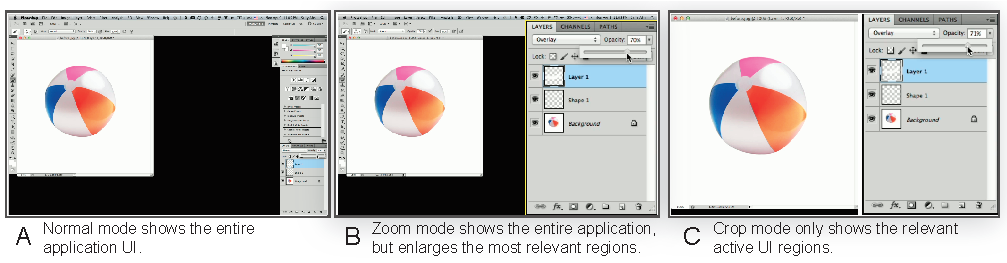
\includegraphics[width=\textwidth]{\mixt/fig/mixt_modes/Fig6}
  \caption{MixT offers three video playback options: Normal mode (A), zoom mode (B) and crop mode (C).}
  \label{fig:mixt_modes}
\end{figure*}

\begin{figure*}[t]
  \centering
  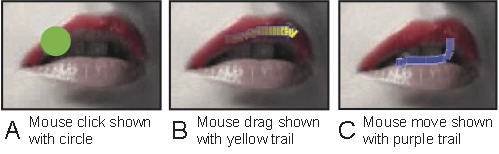
\includegraphics[width=0.7\textwidth]{\mixt/fig/mixt_mouse/mouse_visualizations}
  \caption{Mouse visualization distinguishes moving and dragging.}
  \label{fig:mixt_mouse}
\end{figure*}
